\section{ Launch Trajectories:Wind. constant thrust EOM vert. motion }\label{sec:q4}    


\textit{Consider the flight of a single-stage sounding rocket in a homogeneous gravity field. The rocket starts vertically along a guide rail. The subsequent flight takes place in an atmosphere in which a constant horizontal winds prevails. It is assumed that the rocket is infinitely (statically) stable, meaning that it responds instantly to the impinging airflow. The influence of atmospheric drag may be ignored. Use the following data: \\
guide rail length 50m\\
wind speed 10 m/s\\
rocket initial (total) mass 1000 kg\\
rocket burnout mass 200 kg\\
specific impulse 300s\\
initial thrust load  0 3\\
gravitational acceleration 9.81 m/s2
}

\subsection{Derivation of the Mass equation}

By definition of mass flow (Slides FRM.11): 

\begin{equation}
t = \frac{M_0-M}{m} = \frac{M_0-M}{T/c_{eff}}= \frac{I_{sp}}{\Psi_0}(1-\frac{M}{M_0})
\label{eq:1}
\end{equation}

In our case: 
$$ t = \frac{I_{sp}}{\Psi_0}(1-\frac{M}{M_0}) =  \frac{300}{3}(1-\frac{200}{1000}) = 80 s$$
\subsection{Derivation of the trajectory equation}

The equation of motion while in the rail is: 

\begin{equation}
	M\frac{dV_z}{dt} = T - Mg_0 = mc_{eff} - Mg_0
\end{equation}

Operating and integrating each term, 
\begin{equation}
dV_z = \frac{T}{M} - g_0 = - c_{eff} \frac{dM}{M} - g_0 dt
\end{equation}

\begin{equation}
\frac{dh}{dt} = V_z =  c_{eff} ln(\frac{M_0}{M}) - g_0 t
\label{eq:4}
\end{equation}

If we integrate again, we obtain the altitude at each time (detailed explanation at slides FRM.11 - FRM.13):
\begin{equation}
h= \frac{I_sp^2}{\Psi_0} g_0 \left( \frac{M}{M_0}ln(\frac{M}{M_0}) + 1 - \frac{M}{M_0} \right) - \frac{1}{2}g_0 t^2 
\label{eq:2}
\end{equation}

Substituting \autoref{eq:1} into \autoref{eq:2} and inserting the numerical values for the end of the guide rail, i.e., $h=50m$, and if we call the coefficient $ x = \frac{M_0}{M_e} $  we obtain an ecuation for the mass:

\begin{equation}
h \frac{\Psi_0}{I_{sp}^2g_0}=50 \frac{3}{300^2\times 9.81} = \frac{1}{x}ln(\frac{1}{x}) + 1 - \frac{1}{x} - \frac{1}{2\Psi_0}\left(1-\frac{1}{x}\right)^2
\label{eq:3}
\end{equation}

By solving this ecuation you obtain the value for $x$ (TIP: if you got a CASIO fx-991 or similar, you can plug the equation, insert an estimate value for X, greater than 1 in this case, and press SOLVE. Otherwise, any numerical method or try and guess can work). 
$$x = \frac{M_0}{M_e} = 1.022964 \ \ \ M_e = 977.55 kg$$. 

The final time is: 

\begin{equation}
	t_e = \frac{I_{sp}}{\Psi_0}\left(1-\frac{1}{x}\right) = \frac{300}{3}\left(1-\frac{1}{ 1.022964}\right) =2.2449 s 
\end{equation}

Recalling \autoref{eq:4}, you obtain the final velocity after the rail: 

\begin{equation}
	v_e = I_{sp}g_0 ln(x) -g_0 t_e = 300\times 9.81 ln(1.022964) - 9.81\times 2.2449 = 44.798 m/s
\end{equation}

\subsection{Angle of attack and flight path angle}


\begin{figure}[H]
	\centering
	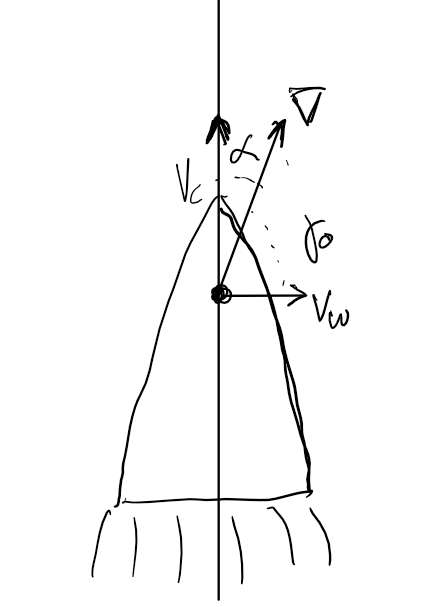
\includegraphics[width=0.3\linewidth]{pics/screenshot002}
	\caption{}
	\label{fig:screenshot002}
\end{figure}

In the instant after leaving the guide rail, the glith path angle is calculated as 

\begin{equation}
	\gamma = atan(\frac{v_e}{v_w}) = atan(\frac{44.798}{10}) = 77,41 \degree
\end{equation}